%%%%%%%%%%%%%%%%%%%%%%%%%%%%%%%%%%%%%%%%%
% Stylish Article
% LaTeX Template
% Version 2.1 (1/10/15)
%
% This template has been downloaded from:
% http://www.LaTeXTemplates.com
%
% Original author:
% Mathias Legrand (legrand.mathias@gmail.com) 
% With extensive modifications by:
% Vel (vel@latextemplates.com)
%
% License:
% CC BY-NC-SA 3.0 (http://creativecommons.org/licenses/by-nc-sa/3.0/)
%
%%%%%%%%%%%%%%%%%%%%%%%%%%%%%%%%%%%%%%%%%

%----------------------------------------------------------------------------------------
%	PACKAGES AND OTHER DOCUMENT CONFIGURATIONS
%----------------------------------------------------------------------------------------

\documentclass[fleqn,10pt]{SelfArx} % Document font size and equations flushed left

\usepackage[english]{babel} % Specify a different language here - english by default
\usepackage{geometry}
\usepackage{lipsum} % Required to insert dummy text. To be removed otherwise

%----------------------------------------------------------------------------------------
%	COLUMNS
%----------------------------------------------------------------------------------------

\setlength{\columnsep}{0.55cm} % Distance between the two columns of text
\setlength{\fboxrule}{0.75pt} % Width of the border around the abstract

%----------------------------------------------------------------------------------------
%	COLORS
%----------------------------------------------------------------------------------------

\definecolor{color1}{RGB}{0,0,0} % Color of the article title and sections
\definecolor{color2}{RGB}{0,20,20} % Color of the boxes behind the abstract and headings

%----------------------------------------------------------------------------------------
%	HYPERLINKS
%----------------------------------------------------------------------------------------
\usepackage{array}
\usepackage{float}
\usepackage{hyperref} % Required for hyperlinks
\hypersetup{hidelinks,colorlinks,breaklinks=true,urlcolor=color2,citecolor=color1,linkcolor=color1,bookmarksopen=false,pdftitle={Title},pdfauthor={Author}}
\geometry{left=1.5cm,right=1.5cm}
%----------------------------------------------------------------------------------------
%	ARTICLE INFORMATION
%----------------------------------------------------------------------------------------

\JournalInfo{ORIE 4741 Final Report} % Journal information
\Archive{Cornell University} % Additional notes (e.g. copyright, DOI, review/research article)

\PaperTitle{Individual Price Prediction for S\&P500 Stocks} % Article title

\Authors{Jiahui Lu(jl3947), Wenjia Zhai(wz363), Yishan Xiong(yx468)} % Authors
%\affiliation{\textsuperscript{1}\textit{Department of Biology, University of Examples, London, United Kingdom}} % Author affiliation
%\affiliation{\textsuperscript{2}\textit{Department of Chemistry, University of Examples, London, United Kingdom}} % Author affiliation
%\affiliation{*\textbf{Corresponding author}: john@smith.com} % Corresponding author

\Keywords{linear regression, random forest, XGBoost} % Keywords - if you don't want any simply remove all the text between the curly brackets
\newcommand{\keywordname}{Keywords} % Defines the keywords heading name

%----------------------------------------------------------------------------------------
%	ABSTRACT
%----------------------------------------------------------------------------------------

\Abstract{The most exciting part of financial investment lies in finding the patterns of price within the uncertainty. In this report, our aim is to find the best machine learning models to predict the stock price of S\&P 500. With the 16 factors we constructed, we used linear models (including Ridge, Lasso and Huber regression), random forest model and XGBoost and compared their performance in the test set. Then we found that the XGBoost gave us the most accurate result using the given data.}
%----------------------------------------------------------------------------------------

\begin{document}

\flushbottom % Makes all text pages the same height

\maketitle % Print the title and abstract box

\tableofcontents % Print the contents section

\thispagestyle{empty} % Removes page numbering from the first page

%----------------------------------------------------------------------------------------
%	ARTICLE CONTENTS
%----------------------------------------------------------------------------------------

%\section*{Introduction} % The \section*{} command stops section numbering
%
%\addcontentsline{toc}{section}{Introduction} % Adds this section to the table of contents
%
%\lipsum[1-3] % Dummy text
% and some mathematics $\cos\pi=-1$ and $\alpha$ in the text\footnote{And some mathematics $\cos\pi=-1$ and $\alpha$ in the text.}.

%------------------------------------------------
\section{Introduction}
\noindent
"Do you want to be the next Buffett?" "5 minutes to show you Soros's trading strategy." Maybe this looks like advertising a lot, sure, you can also understand them as advertising for our project. In fact, I don't have to start this way. Forecasting the stock price itself is an idea easy to be understood, but in case you get bored for this, maybe I need more explanation. Predicting stock prices has clearly become one of the most popular topics for a long time, People who want to get rich overnight are always more inclined to financial markets, as “money never sleep” while they get enough money and enough sleeps. What's more interesting is that this topic is so popular that it starts to be boring( which may also be the reason why the interesting part of our opening peer review only scored 3.5 points)...\\
\newline
\noindent
In fact, no one can reject this thirst for wealth in the blood, and what this project does is the first step in using big data technology to succeed in the financial world. We believe everyone has such a moment when you sit in front of your computer and stare at the changing stock price curve on the screen, guessing where it will go in the next second, and suddenly wake up and say to yourself: stop dreaming! There is no way to get rid of those complex financial statements if you want to make money! What can be done only with stock prices and trading volume? The idea of our project is to tell everyone that this is not a dream. With the help of machine learning models such as linear models (including Ridge, Lasso and Huber regression), random forest model and XGBoost, only simple historical data can be used to predict the stock price.
%------------------------------------------------
\section{Data Exploration} % The \section*{} command stops section numbering

\subsection{Data Overview}
We wish to predict the S\&P 500 component stocks' prices. The S\&P 500 stock market index, maintained by S\&P Dow Jones Indices, comprises 505 common stocks issued by 500 large-cap companies and traded on American stock exchanges.At the same time, we divided them into 54 groups according to the industries they belong to. \\ 
\newline
\noindent
Our raw data comes from Wharton database, with a time span of 10 years and 505 stocks in total. The data contains:
\begin{enumerate}%[noitemsep]
    \item \textbf{Daily stock prices} include open price, bid price and ask price with their bound prices
    \item \textbf{Return values} include holding period return and return without dividends.
    \item \textbf{Trading volumes} is the number of shares traded in a day.
    \item \textbf{VIX Index} is a popular measure of the stock market's expectation of volatility implied by S&P 500 index options.
    \item \textbf{Industry} is the industry category that each stock belongs to.
\end{enumerate}
\noindent
For the sample data set, please refer to the Appendix file in our Github folder. 
 


\subsection{Data Preprocessing}
\noindent
The data we were processing is quite messy with different ratio of missing data. Sometimes the missing data is distributed separately, while sometimes they are lost for a whole period of time. Here for separated missing data, we didn't fill in the empty ones since our factors don't have actual value in the missed date, though we can calculate it out. This may cause huge problems if we want to use it in real trades. Thus, we drop the empty values. The continuous period for missing values is also possible to exist for two reasons: First is that there may be a period of time that the stock stopped trading; Second, the S\&P 500 stock components i always changing. Sometimes the stock is dropped out or added into the portfolio. Because our aim is to predict the individual stock's price, so in order to keep the sample as large as possible, if a stock has less than 2000 obs, then we drop it from our data set. \\

\newline
\noindent
Then we divided the stocks according to the industry, since we believe that stocks in the same industry may have similar patterns. Here we met another problem: the industry that a stock belongs to can change over time. Thus, we divided the data dynamically, which means we divided the stocks with the industry they belong to in that period. As the period ends, we divided the stock again.\\
\newline
\noindent
As the modeling logic is the same, and it would be a mess if we show all 500 stocks here, we chose 1 stock from each industry randomly using Pseudo-random number and visualized the output in this report. For a stock whose industry has changed, if the numbers of obs in each industry are all less than 2000, we won't choose this stock since it can not represent the industry well.


%------------------------------------------------
\section{Features}

\subsection{Feature Engineering}

\begin{table*}[t]
  \centering
\caption{Feature Descriptions}
\begin{tabular}{p{0.1\columnwidth}|p{0.8\columnwidth}|p{0.9\columnwidth}} 
      \hline
      Feature ID & Formula (all features are delayed by 1day in our real calculation) & Descriptions \\
      \hline
      1	& Mean(((Close-Low)-(High-Close))/(High-Low)*Volume, 20)/Volume & A measure of the mean intraday level of close price, modified by volume.\\
      \hline
      2 & (High-Mean(High,5))/Mean(High,5) & A comparison between today's high price and the previous mean.\\
      \hline
      3 & Std(Volume,20)/Volume & A measure of the monthly volume dispersion.\\
      \hline
      4 & (Ask-Bid)/(Delay(Ask,1)-Delay(Bid, 1)) & The change of bid-ask spread.\\
      \hline
      5 & Corr(Rank(Close), Rank(Volume), 10) & The deviation or converge of close price and volume using their market level.\\
      \hline
      6 & (((High*LOW)**0.5)-Close)/Close & A comparison between close price and the “geometric mean” intraday price. \\
      \hline
      7 & 1-Close/Delay(Close, 5) & A feature to measure the inverse effect of stock price.\\
      \hline
      8 & Rank(Std(High, 10)) & A market level measurement of high price fluctuation.\\
      \hline
      9 & tsMax(Corr(tsRank(Volume, 5), tsRank(Close, 5), 5),3) & The time series max of the deviation or converge of close price and volume.\\
      \hline
      10 & 1-VWRET/Delay(VWRET, 5) & The value-weighted return change.\\
      \hline
      11 & Std(Close, 5)/Close & A measure of the weekly close price dispersion.\\
      \hline
      12 & Corr(High, Volume, 10) & The deviation or converge of high price and volume trend.\\
      \hline
      13 & Std(VWRET, 20)/VWRET & A measure of the monthly return dispersion.\\
      \hline
      14 & Mean(High/Low, 20) & A measure of individual stock price volatility.\\
      \hline
      15 & VIX Index & The CBOE Volatility Index. A popular measure of the stock market's expectation of volatility.\\
      \hline
      16 & Industry Index Quote & The pseudo prices of each industry index calculated by the equally-weighted-average of member stocks' prices. \\
      \hline
  \end{tabular}
  \label{tab:2}
\end{table*}

\subsubsection*{Idea Generation}
In quantitative investment world, there exist various ways to seek for valid signals from the stock market to predict the future price. To simplify the problem, we mainly look into the stock's previous price, volume, volatility in our project, and use these data to generate formula signals which reflect some kind of investment theories people believe in.
\subsubsection*{Price and Volume Correlation}
The theory is that when price and volume move together, the stock is "acting" correctly. Therefore, the higher the correlation, the better acting the stock is. If the correlation is strongly negative, we may see a constructive short forming. More specifically: 
\noindent
\begin{enumerate}
    \item If the stock price and volume change in the same direction: The rise in the stock price and the increase in trading volume shows that people keep believing in positive performance of the market; the decline in price as well as the volume indicates that people are optimistic about the future market outlook, holding positions and waiting.
    \item If the stock price and volume show opposite changes. The rise of the stock price and the decrease of the volume indicate that the upward trend of the stock price cannot be supported by the transaction volume, and makes the trend difficult to maintain; the decline in the stock price with the increase in the transaction volume is an indicator of the downturn in the market.
\end{enumerate}

\noindent
We try to capture this theory in different forms and meanings with feature 1,5,9,12.

\subsubsection*{Momentum \& Reverse Effect}
Momentum is the empirically observed tendency for rising asset prices to rise further, and falling prices to keep falling. Momentum signals have been widely used by financial analysts in their buy and sell recommendations. Reverse Effect is the opposite belief with the Momentum Effect.\\
\noindent
We try to capture this effect with feature 2, 7, 10.

\subsubsection*{Stock Volatility \& Market Volatility}
Stock market volatility is generally associated with investment risk. Volatility is most traditionally measured using the standard deviation, which indicates how tightly the price of a stock is clustered around the mean or moving average. Larger standard deviations point to higher dispersion of returns as well as greater investment risk. \\
\newline
\noindent
 Usually, volatility increases as stock prices decline, and volatility declines as stock prices increase. The reason is presumably because falling stock prices mean deteriorating business conditions, and deteriorating business conditions mean higher risk from worsened visibility. This leads to greater daily price fluctuations (on a percentage basis) and thus, greater volatility. On the other hand, as stock prices climb, this implies improving business conditions and greater stability. Thus, stocks exhibit smaller daily price fluctuations, i.e., lower volatility. In addition, we assume that the market volatility also can be an indication for individual stock.\\
\newline
\noindent
We try to capture this phenomenon with feature 8, 11, 13, 14 (stock volatility), 15(market volatility).

\subsubsection*{Other}
We also add some features about volume dispersion (feature 3), bid-ask spread (feature 4), intraday-change (feature 6), industry performance (feature 16) in our model to add more explanatory power.\\

\begin{figure}[htb]\centering % Using \begin{figure*} makes the figure take up the entire width of the page
\includegraphics[width=\linewidth,height=6cm]{feature_distribution.png}
\caption{Feature Distribution}
\label{fig:view}
\end{figure}

\noindent
To make it easier to find the characteristics of our data, we randomly select one single company with the ticker "MO" as an example.\\
\newline
\noindent
From Figure 1.Feature Distribution , we can see feature 1,2,4,5,6,7,\\
10,11,12,13,16 look like the normal distribution very much, and feature 3,8,9,14,15 follow skewed distribution.\\

\subsection{Feature Selection}

\subsubsection*{Feature relationship}

\begin{figure}[ht]\centering % Using \begin{figure*} makes the figure take up the entire width of the page
\includegraphics[width=\linewidth,height=6cm]{heatmap.png}
\caption{Heatmap of Feature Correlation}
\label{fig:view}
\end{figure}

From Figure 2. Heatmap, we can see that feature2 \& feature7, feature5 \& feature12, feature6 \& feature16, feature14 \& feature15 have a relative high correlation. Among them, feature2 \& feature7 has the largest correlation, which is -0.84, and other pairs' correlations are all smaller than 0.62, which we see as acceptable in our project. \\
\newline
In this case, we dropped \textbf{feature2} and keep feature7. One reason is because feature7 can give us a more direct and clear financial explanation, another reason is feature7 follows a distribution much more closer to a normal distribution.
%------------------------------------------------
%newpage
\section{Model Selection}
\subsection{Linear Models}
In this part, we used linear model with different loss functions and different regularizers, to see how well the linear model can predict our target. The logic is simple. The first step is dividing the data set into training set and testing set. Because our data is time series data, the cross validation method is useless since we can't use the future data to predict the historical ones. Thus, we should divide the data according to the time order. Here we divided it into training set(75\%) and test set(25\%). Then we used Linear regression including Ridge regression, Lasso regression and Huber regression by training them separately and then used their parameters that performed the best in training set into test set.  \\


\subsubsection{Ridge regression}
The first model we tried was \textbf{ridge regression}:
$$ \text{minimize} \quad \sum_{i=1}^{n} (y_i - w^Tx_i)^2 + \lambda \sum_{i=1}^{n} {w_i}^2$$
The ridge could help us prevent the problem of overfitting thanks to $l_2 $ square deviation factor. As we know, the ridge regression may add a little bit bias but can reduce the risk of overfitting (crazy outcomes) significantly and thus performs better when predicting test set. Besides, when given very different input data, the ridge regression can prevent some "crazy" prediction. By plotting out the MSE value based on different $\lambda s$, we found the optimal $\lambda s$ and then we applied them into the models and saw the result in the test sets. \\
\newline
\noindent
As our data includes more than 500 stocks, it would be messy if we plot their performance together. Thus, we randomly chose 2 stocks whose tickers are "IRM" and "LNC". To better estimate the parameters, we tried $\lambda$ from 0 to 3 with the step size 0.1. Here is the plots of MSE results of test sets given $\lambda$. The orange spot shows the best solution of $\lambda$ we chose for its best performance in the training set. The blue spot shows the actual best $\lambda$ which can give us the lowest MSE in the testset. \\

\begin{figure}[ht]\centering % Using \begin{figure*} makes the figure take up the entire width of the page
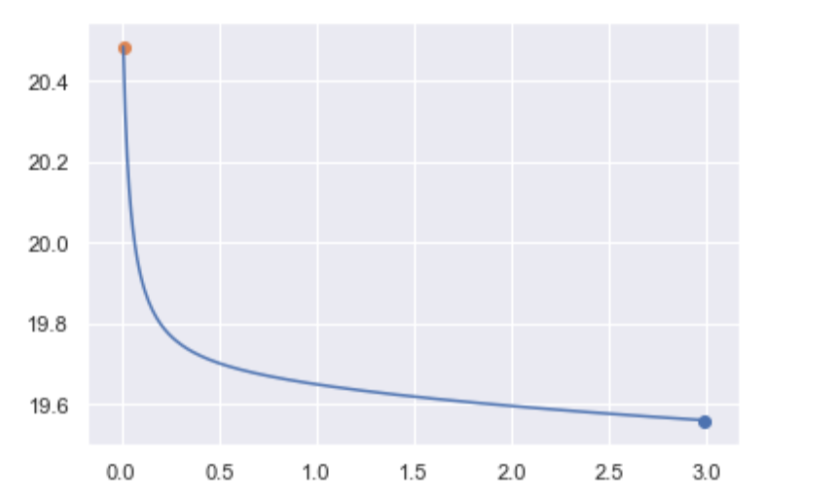
\includegraphics[width=\linewidth]{irm_ridge.png}
\caption{Select $\lambda$ for IRM Ridge Regression}
\label{fig:view}
\end{figure}

\begin{figure}[ht]\centering % Using \begin{figure*} makes the figure take up the entire width of the page
\includegraphics[width=\linewidth]{Lnc_ridge.png}
\caption{Select $\lambda$ for LNC Ridge Regression}
\label{fig:view}
\end{figure}

\noindent
From fig.3 and fig.4, we can see that for different stocks, their MSE curves' shapes are really different. For IRM company, the MSE curve according to $\lambda$ is decreasing continuously until it converges to a certain value (here is approximately 19.6). That shows that the ridge regression can improve the result of linear regression significantly . However, our model used a relatively small $\lambda$. In the LNC company's situation, the curve is not decreasing continuously. On the contrary, MSE has a minimum point near $\lambda$=1.7. After that, the MSE goes up. That may because a more severe punishment makes the parameter even smaller than it should be, and the model thus cannot explain the price change enough. Also we can find that the $\lambda$ we selected is far smaller than the actual best $\lambda$. This shows that it might be difficult for us to estimate the best $\lambda$.\\
\newline
\noindent
After that, we can also draw the picture of the coefficients value changes according to the $\lambda$.\\

\begin{figure}[ht]\centering % Using \begin{figure*} makes the figure take up the entire width of the page
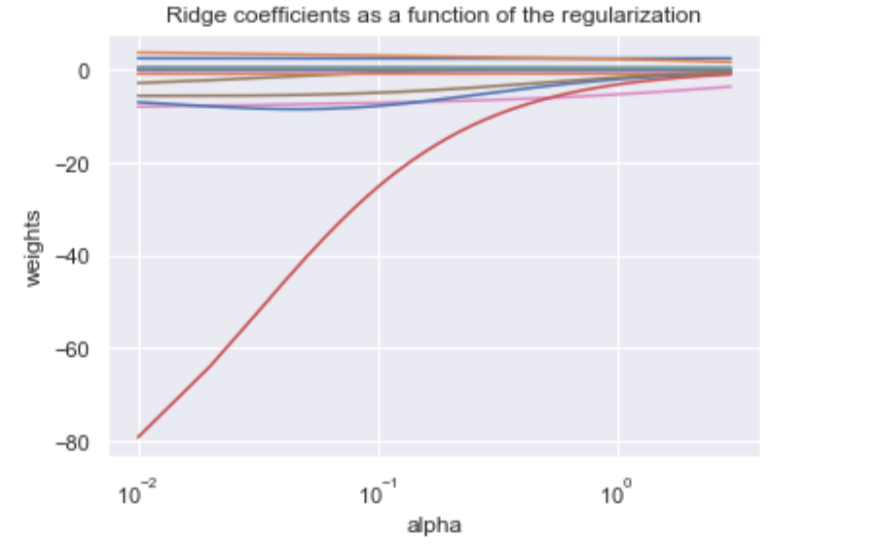
\includegraphics[width=\linewidth]{irm_ridge_alpha.png}
\caption{Coefficients for IRM Ridge Regression}
\label{fig:view}
\end{figure}

\begin{figure}[ht]\centering % Using \begin{figure*} makes the figure take up the entire width of the page
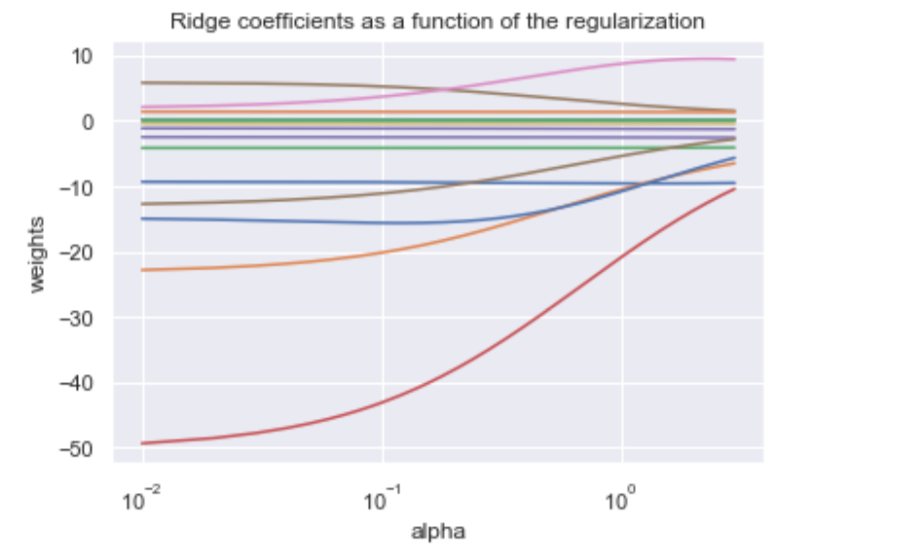
\includegraphics[width=\linewidth]{lnc_ridge_alpha.png}
\caption{Coefficients for LNC Ridge Regression}
\label{fig:view}
\end{figure}
\noindent
From fig.5 and fig.6, we can see that most of the coefficients of both stocks follow a decreasing trend as the $\lambda$ rising. That's reasonable since the punishments for big coefficients become huge as $\lambda$ grows. We can also see that in both graphs there are factors that used to have extremely large absolute value. That may cause what we called a 'crazy' prediction. Thus the ridge regression is really useful when solving the problem of overfitting.

\subsubsection{Lasso regression}
\noindent
We also tried \textbf{lasso regression}:
$$ \text{minimize} \quad \sum_{i=1}^{n} (y_i - w^Tx_i)^2 + \lambda \sum_{i=1}^{n} |w_i|$$
The lasso regularizer usually tend to give a more sparse result. That is to say, when the ridge regression has many parameters that are close to 0, the lasso can just make them to 0 which costs us less time in calculation. We can use this property to select an appropriate subset of features for the prediction, and that also increases the model accuracy. To better compare with the ridge model, we use the same 2 stocks for comparison.\\

\begin{figure}[ht]\centering % Using \begin{figure*} makes the figure take up the entire width of the page
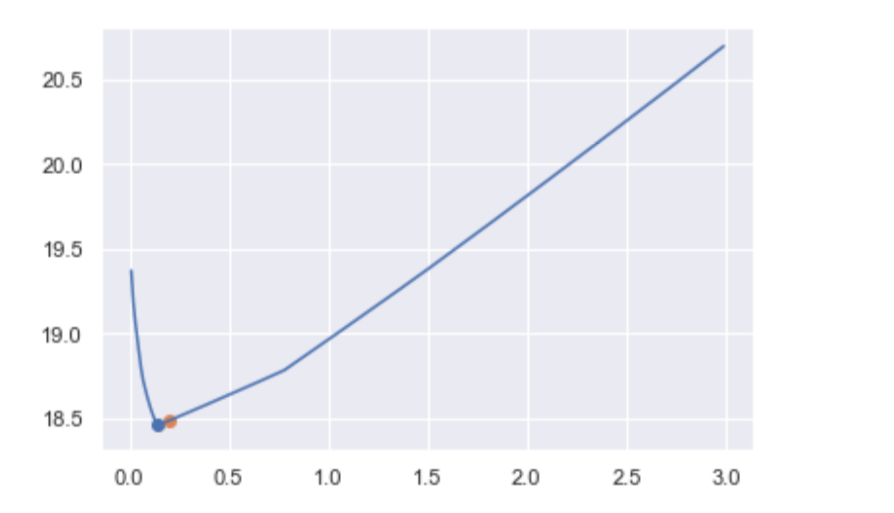
\includegraphics[width=\linewidth]{irm_lasso.png}
\caption{Select $\lambda$ for IRM Lasso Regression}
\label{fig:view}
\end{figure}

\begin{figure}[ht]\centering % Using \begin{figure*} makes the figure take up the entire width of the page
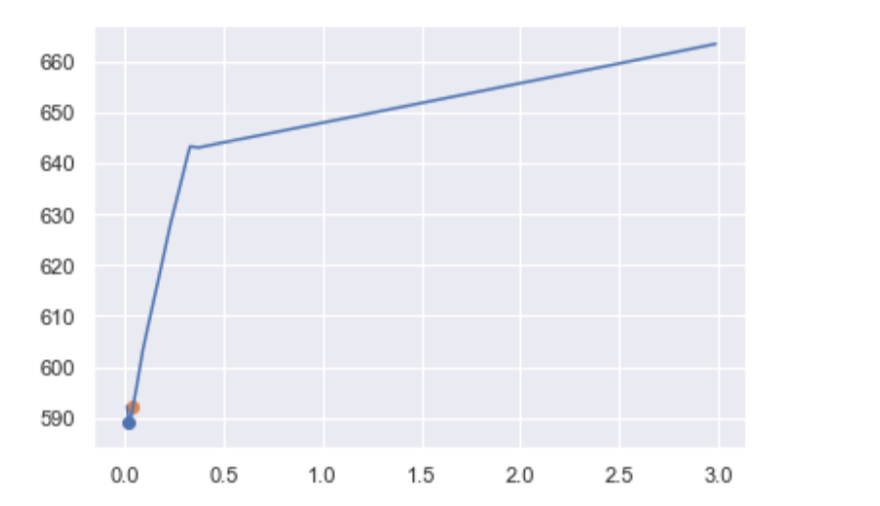
\includegraphics[width=\linewidth]{lnc_lasso.png}
\caption{Select $\lambda$ for LNC Ridge Regression}
\label{fig:view}
\end{figure}

\noindent
From fig.7 and fig.8, we are surprised to find that the shapes of curves are totally different, as the LNC company's MSE is getting higher as the $\lambda$ grows while the IRM's MSE has a minimum point. The good news is that the $\lambda$ we selected this time is really close to the best $\lambda$, which means it may be easier to estimate the parameter $\lambda$ in the Lasso regression.\\

\begin{figure}[ht]\centering % Using \begin{figure*} makes the figure take up the entire width of the page
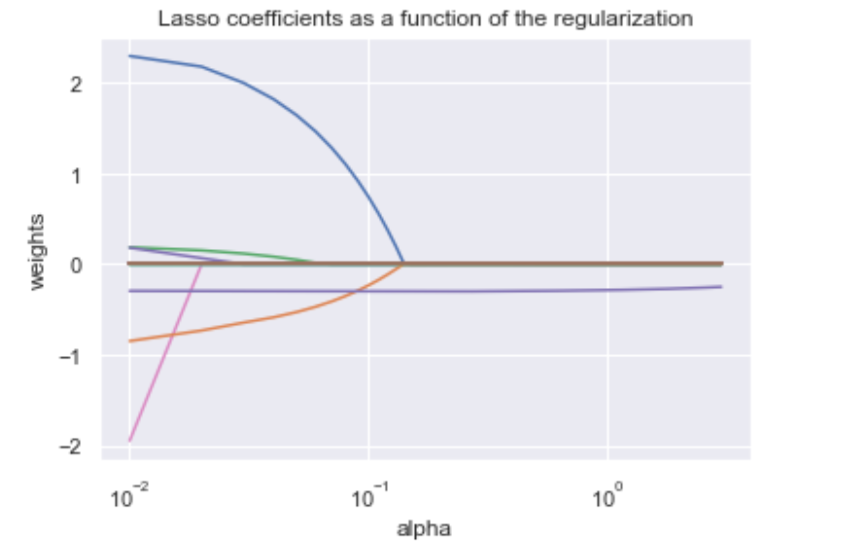
\includegraphics[width=\linewidth]{irm_lasso_alpha.png}
\caption{Coefficients for IRM Lasso Regression}
\label{fig:view}
\end{figure}

\begin{figure}[htb]\centering % Using \begin{figure*} makes the figure take up the entire width of the page
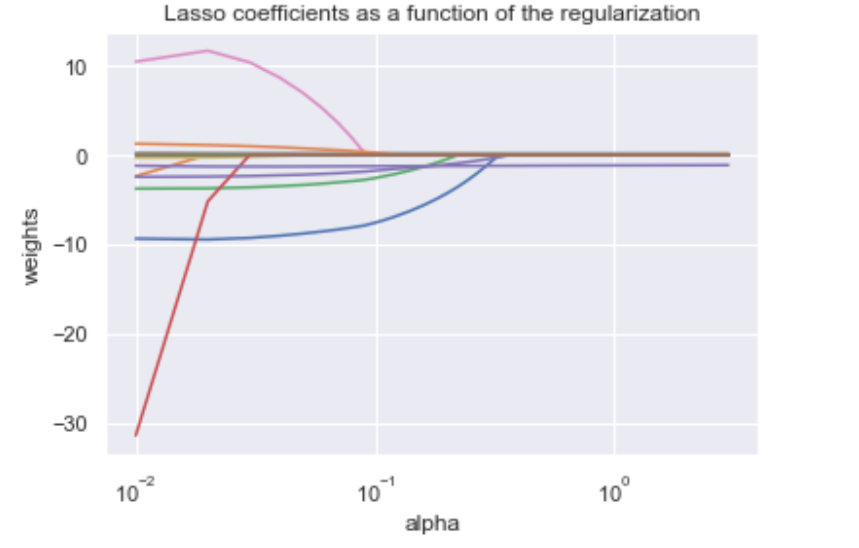
\includegraphics[width=\linewidth]{lnc_lasso_alpha.png}
\caption{Select $\lambda$ for LNC Lasso Regression}
\label{fig:view}
\end{figure}

\noindent
From fig.9 and fig.10, we can easily find in the graphs that using Lasso Regression, the solution is sparse: as the $\lambda$ rising, some of the coefficients become 0. That explains why the MSE curve going up forward: if $\lambda$ goes higher than a certain point, nearly all coefficients go to 0. That point value is less than 0.1. But we shouldn't worry about the number of the factors, since for the $\lambda$ we selected there are still more than 10 factors exist. That also tell us we should find a balance between cutting off and persisting in these factors. Making the matrix more and more sparse is not always a good idea.

\subsubsection{Huber regression}
The third linear model we used is the \textbf{huber regression}:
$$ \text{minimize} \quad \frac{1}{n}\sum_{i=1}^{n} \textbf{huber}(y_i - w^Tx_i)$$

$$
\textbf{huber}(z) = \left\{
\begin{array}{rcl}
\frac{1}{2}z^2 && |z| \le \epsilon \\
|z| - \frac{1}{2} && |z| \ge \epsilon \\ 
\end{array}
\right.
$$

\noindent
The huber loss is calculated as a combination of squared loss and absolute loss. Huber Loss combines MSE and MAE losses. Using MSE when the error is close to 0 makes the loss function differentiable and the gradient becomes more stable. Using MAE when the error is large can reduce the impact of the outliers and makes the training more robust to the outliers. The disadvantage is that an extra parameter $\epsilon$ needs to be set. So to find the best parameter, we tested all the numbers in [1,3) by 0.1. The following plot shows how the best $\epsilon$ of the 54 stocks is distributed. Note that here we only have 51 stocks available since some of the stocks are not converged in the given time. The best $\epsilon$ distribution is as follows:  

\begin{figure}[ht]\centering % Using \begin{figure*} makes the figure take up the entire width of the page
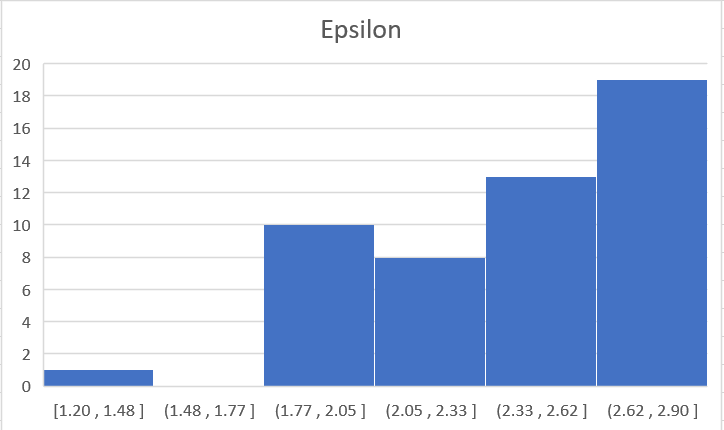
\includegraphics[width=\linewidth]{epsilon.png}
\caption{Select parameters for huber regression}
\label{fig:view}
\end{figure}
\noindent
From fig.11, we can see that although the frequency is largest between [2.62,2.9], the $\epsilon$ occurs not only at the maximum. When $\epsilon$ is large, then the Huber regression is actually the same as the linear regression. Thus, this histogram shows that it is different than the linear regression. Huber is effective. \\

\subsection{Random Tree Model}
In this project, we utilized random forest model to predict the price of the stock. Random forest is an ensemble learning method that operates by constructing a multitude of decision trees at training time and outputting the mean prediction value of the individual trees.\cite{Breiman2001}\\
\newline
\noindent
First of all, we split the whole dataset into two part, the 75th percentile as train set and the rest as test set. Then, we created the single tree by randomly picking $max\_feature$ from total 16 features and splitting the dataset into two parts which have the minimum sum value of mean square error.  We repeated this process $max\_depth$ times to create the single tree. Then, we created $n\_estimators$ trees to form the forest. After the training process, each tree will make a prediction based on the new input data. Finally, we took the average prediction of all decision trees as the output of the random forest model.\\

\begin{figure}[ht]\centering
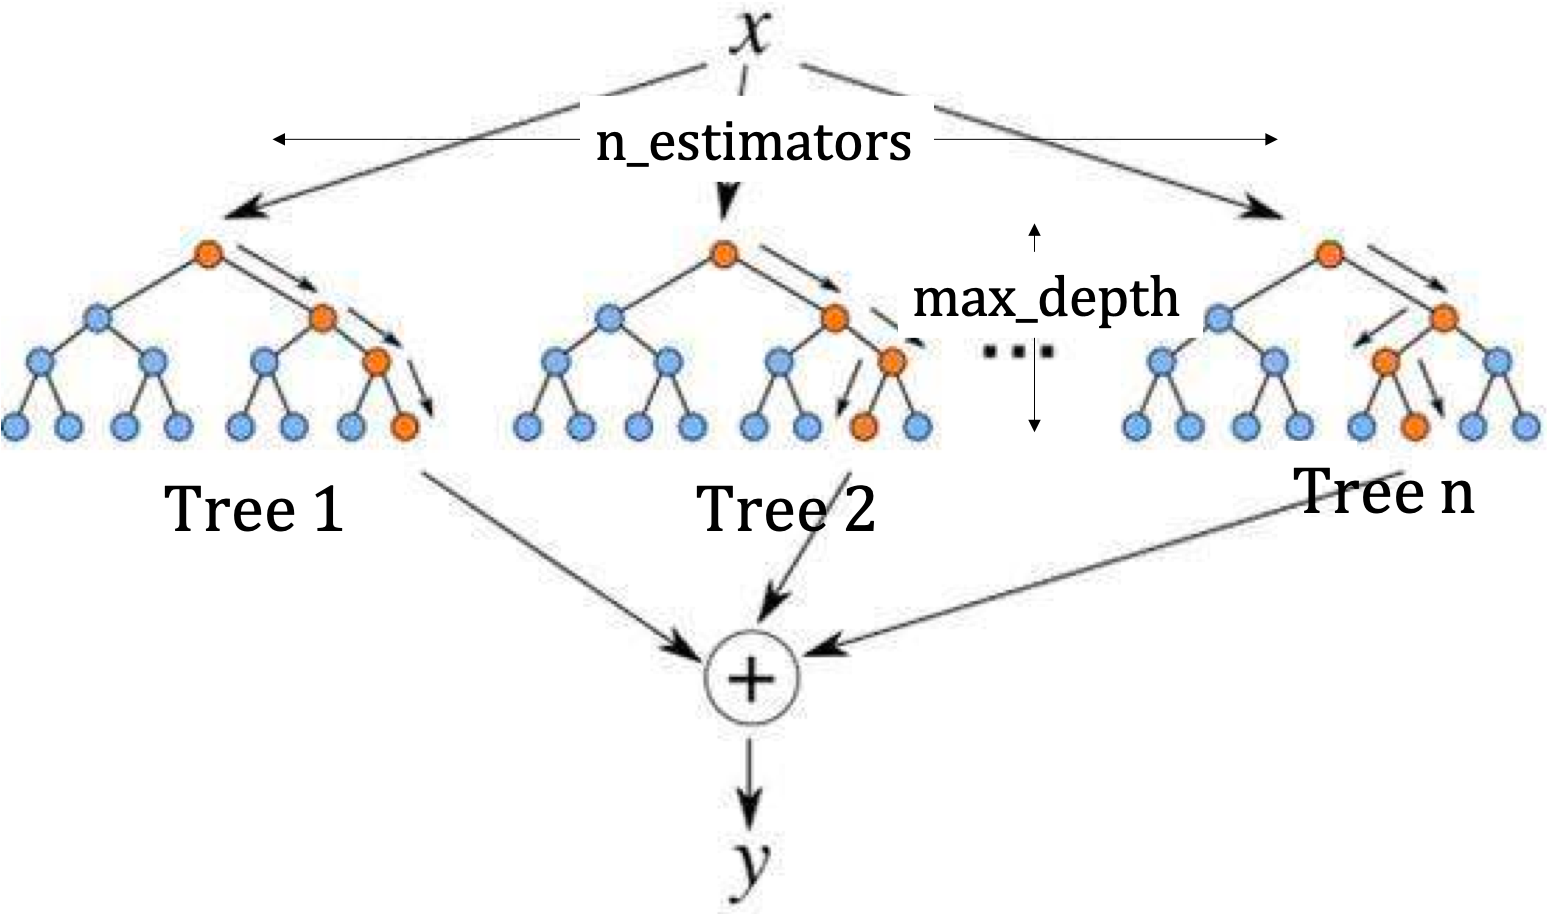
\includegraphics[width=\linewidth]{random_tree_process.png}
\caption{Random Forest Process}
\label{fig:results}
\end{figure}

\begin{figure}[ht]\centering % Using \begin{figure*} makes the figure take up the entire width of the page
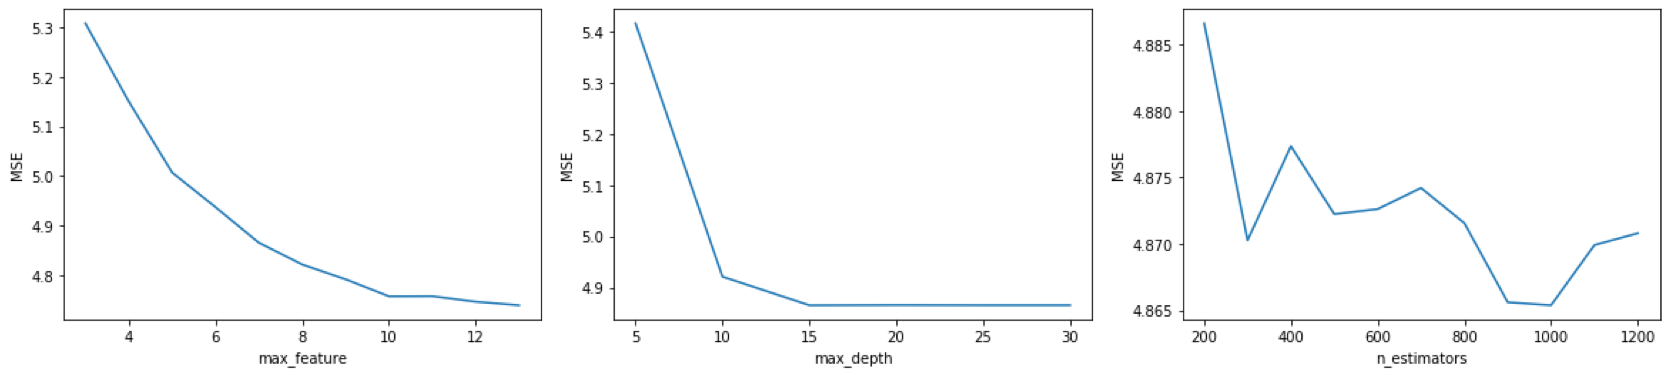
\includegraphics[width=\linewidth]{random_forest_para.png}
\caption{Random forest parameters}
\label{fig:view}
\end{figure}

\noindent 
For random forest model, there are 3 parameters, $max\_feature$, $max\_depth$ and $n\_estimators$. To find the optimal parameters for each stock, first of all, we randomly pick one stock to find the trend of each parameters. \\
%\begin{figure}[ht]\centering
%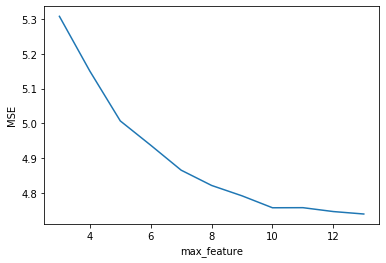
\includegraphics[width=\linewidth]{max_ft.png}
%\caption{$max\_feature$ Trend}
%\label{fig:results}
%\end{figure}
%
%\begin{figure}[ht]\centering
%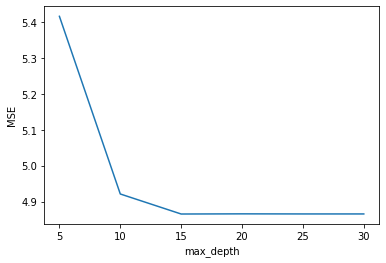
\includegraphics[width=\linewidth]{max_dp.png}
%\caption{$max\_depth$ Trend}
%\label{fig:results}
%\end{figure}
%
%\begin{figure}[ht]\centering
%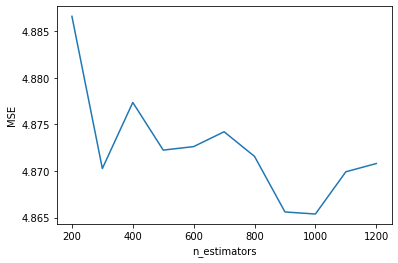
\includegraphics[width=\linewidth]{n_est.png}
%\caption{$n\_estimators$ Trend}
%\label{fig:results}
%\end{figure}
%


\noindent 
From Figure 13, we can see that for $max\_feature$, MSE is going to decrease as $max\_feature$ increase. For running time consideration, we will test $max\_feature$ as 7, 8, 9 and 10 to find the optimal parameter of $max\_feature$. For $max\_depth$, MSE is going to be a constant when $max\_depth$ is large enough. In this way, we will test $max\_depth$ as 15,20 and 25 to find the optimal parameter of $max\_depth$. For $n\_estimators$, MSE is fluctuated and reached the minimum value at 1000. In this way, we will test $n\_estimators$ as 800,900,1000 and 1100 to find the optimal parameter of $n\_estimators$.\\

\subsection{Comparison}
For 54 stocks we selected, we compare each model's MSE and find the model which provides least MSE. The result can be seen in the figure 14. On testing set, random forest model has the lowest MSE for 33 stocks, which performs better than linear models. This is because the random forest model can better describe the non-linear relation between the input and output data and the features we selected has non-linear relation with stock price. \\
\newline
And for linear models, ridge model has the lowest MSE for 13 stocks, which performs better than other two linear models. That lasso only has 1 lowest MSE for stock is because lasso model can only use numerical method to approximate the result since it can't obtain explicit solution as ridge and huber model. And since huber is less sensitive than ridge model to higher volatility in dataset, huber model performs worse than ridge model in predicting stock price. \\
\newline
\begin{figure}[ht]\centering
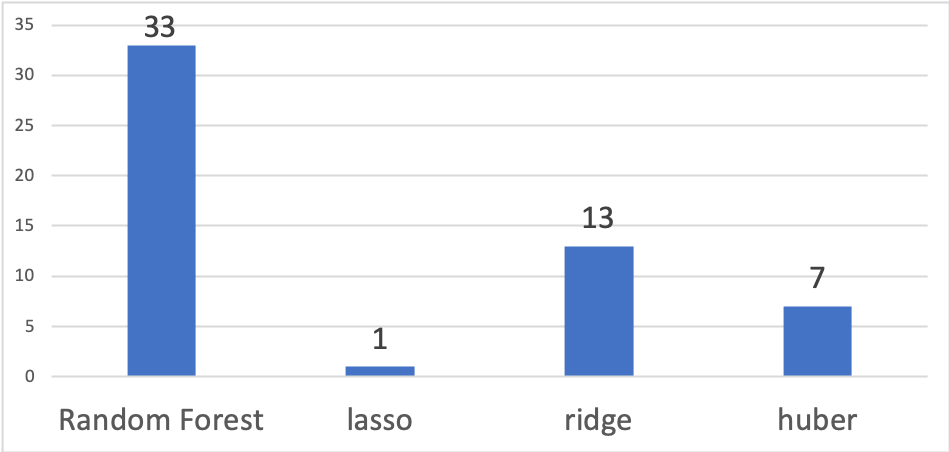
\includegraphics[width=\linewidth]{compare1.png}
\caption{Model provide least MSE}
\label{fig:results}
\end{figure}
\noindent

\subsection{XGBoost Model}

\noindent
\textbf{Boosting} is an ensemble technique where new models are added to correct the errors made by existing models. In boosting, the individual models are not built on completely random subsets of data and features but sequentially by putting more weight on instances with wrong predictions and high errors. The model learns from past mistakes.\cite{xgboost}\\
\newline
\noindent
\textbf{Gradient boosting} is an approach where multiple models are created that predict the residuals or errors of prior models and then added together to make the final prediction. It is called gradient boosting because it uses a gradient descent algorithm to minimize the loss when adding new models. \\
\newline
\noindent
\textbf{XGBoost} stands for Extreme Gradient Boosting; it is a specific implementation of the Gradient Boosting method which uses more accurate approximations to find the best tree model. It has recently been dominating applied machine learning and Kaggle competitions for structured or tabular data. \\

\begin{figure}[ht]\centering % Using \begin{figure*} makes the figure take up the entire width of the page
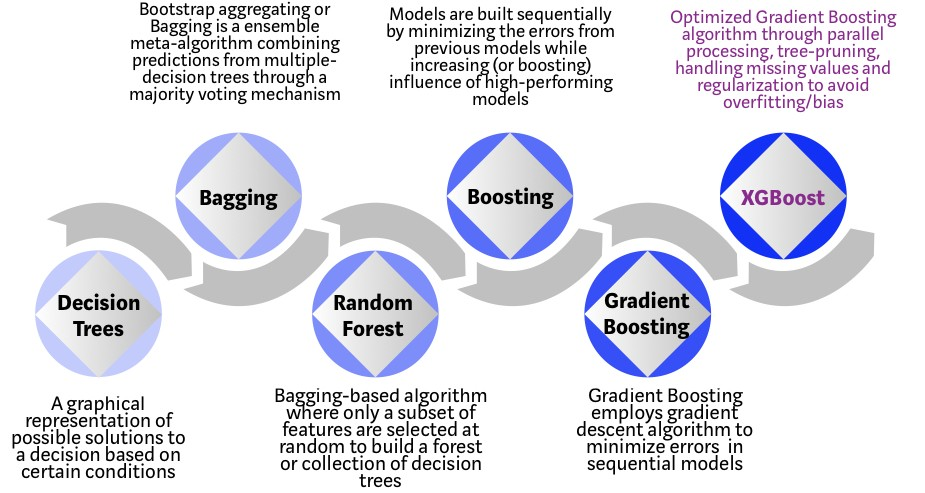
\includegraphics[width=\linewidth,height=4cm]{evolution.jpeg}
\caption{Evolution of XGBoost Algorithm}
\label{fig:view}
\end{figure}

\noindent
In our project, we used the open source Python package XGBoost to fit the model. It has several parameters to customize:\\
(a) learning rate: The “step size” with which we descend the gradient.\\
(b)  n estimators: The number of trees (or rounds) in an XGBoost model.\\
(c)  max depth: The maximum depth of a tree. Used to control over-fitting as higher depth will allow model to learn relations very specific to a particular sample.\\
(d)  min child weight: Defines the minimum sum of weights of all observations required in a child. Used to control over-fitting. \\
(e)  gamma: A node is split only when the resulting split gives a positive reduction in the loss function. Gamma specifies the minimum loss reduction required to make a split. \\
(f) reg alpha: L1 regularization term on weight. Can be used in case of very high dimensionality so that the algorithm runs faster when implemented.\\
(g)  reg lambda: L2 regularization term on weights (analogous to Ridge regression) This used to handle the regularization part of XGBoost and to reduce overfitting.\\


\noindent
It is difficult to get a very big leap in performance by just using parameter tuning. So we just make a rough optimization. Randomly, we picked the stock with ticker 'MO', and used it as an example to decide the optimal range of these parameters. The result is shown in the following chart and graphics. In order to save time and resources, we narrowed down the parameters' range and even fixed some parameters.  

\begin{table}[h]
  \centering
\caption{Parameters Range}
\begin{tabular}{ |c|c|c| }
      \hline
      Parameters & Value & Description\\
      \hline
      learning rate & [0.025, 0.05, 0.075] & Search Range\\
      \hline
      n estimators & 500 & Fixed Value\\
      \hline
      max depth & [5, 6, 7, 8, 9] & Search Range\\
      \hline
      min child weight & [5, 6, 7, 8] & Search Range\\
      \hline
      gamma & [0.2, 0.3, 0.4] & Search Range\\
      \hline
      reg alpha & 0.1 & Fixed Value\\
      \hline
      reg lambda & 1 & Fixed Value \\
      \hline
  \end{tabular}
  \label{tab:2}
\end{table}
\noindent
Then we utilized the function $GridSearchCV$ from the package $sklearn.model_selection$ to travel the numbers in the range we narrowed down and finally found the optimized parameters for each stock (model). And we used the best model on training set to predict on the test set, and calculated the MSE of each stock's prediction model.

\begin{figure}[hbtp]\centering % Using \begin{figure*} makes the figure take up the entire width of the page
\includegraphics[width=\linewidth,height=4.5cm]{xgboost_combine.png}
\caption{Parameters Selection}
\label{fig:view}
\end{figure}


%\begin{figure}[ht]\centering % Using \begin{figure*} makes the figure take up the entire width of the page
%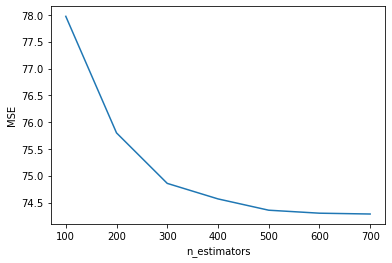
\includegraphics[width=\linewidth,height=4.5cm]{n_estimators.png}
%\caption{n estimators Selection}
%\label{fig:view}
%\end{figure}
%
%\begin{figure}[ht]\centering % Using \begin{figure*} makes the figure take up the entire width of the page
%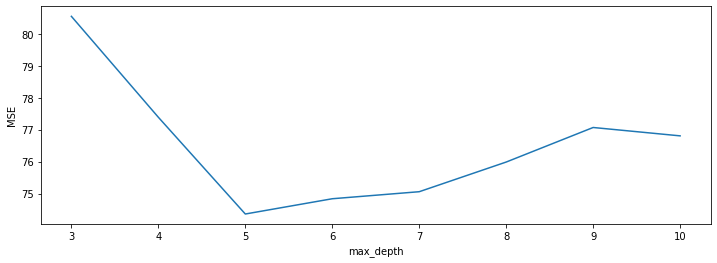
\includegraphics[width=\linewidth,height=4.5cm]{max_depth.png}
%\caption{max depth Selection}
%\label{fig:view}
%\end{figure}
%
%\begin{figure}[ht]\centering % Using \begin{figure*} makes the figure take up the entire width of the page
%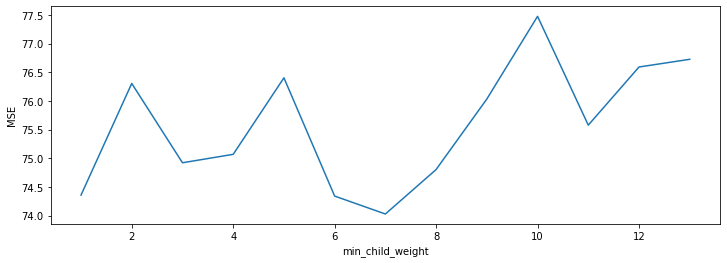
\includegraphics[width=\linewidth,height=4.5cm]{min_child_weight.png}
%\caption{min child weight Selection}
%\label{fig:view}
%\end{figure}
%
%\begin{figure}[ht]\centering % Using \begin{figure*} makes the figure take up the entire width of the page
%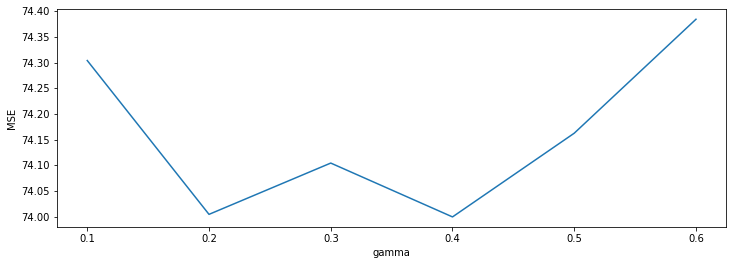
\includegraphics[width=\linewidth,height=4.5cm]{gamma.png}
%\caption{gamma Selection}
%\label{fig:view}
%\end{figure}
%
%\begin{figure}[ht]\centering % Using \begin{figure*} makes the figure take up the entire width of the page
%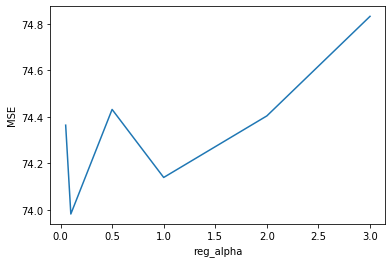
\includegraphics[width=\linewidth,height=4.5cm]{reg_alpha.png}
%\caption{reg alpha Selection}
%\label{fig:view}
%\end{figure}
%
%\begin{figure}[ht]\centering % Using \begin{figure*} makes the figure take up the entire width of the page
%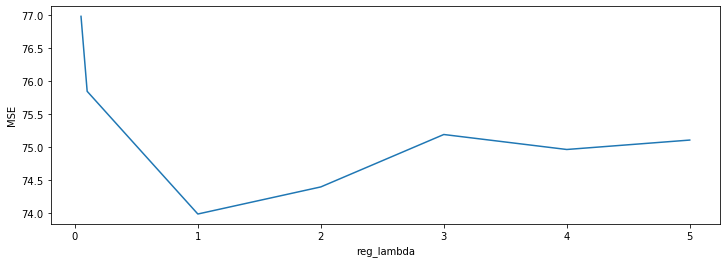
\includegraphics[width=\linewidth,height=4.5cm]{reg_lambda.png}
%\caption{reg lambda Selection}
%\label{fig:view}
%\end{figure}
%
%\begin{figure}[ht]\centering % Using \begin{figure*} makes the figure take up the entire width of the page
%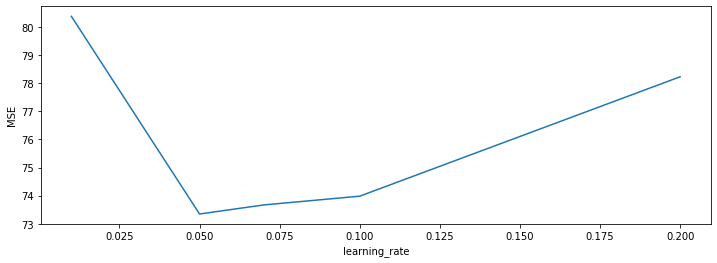
\includegraphics[width=\linewidth,height=4.5cm]{learning_rate.png}
%\caption{learning rate Selection}
%\label{fig:view}
%\end{figure}



\subsection{Compare}
After we introduced XGBoost model, we found out that XGBoost performed better than random forest model and linear models. This is because XGBoost's loss function is second Taylor expansion of error, which is more precise than other models. And XGBoost improves the random forest model by using regularization to control over-fitting. In this way, XGBoost would perform much better than other models we used. \\

\begin{figure}[ht]\centering
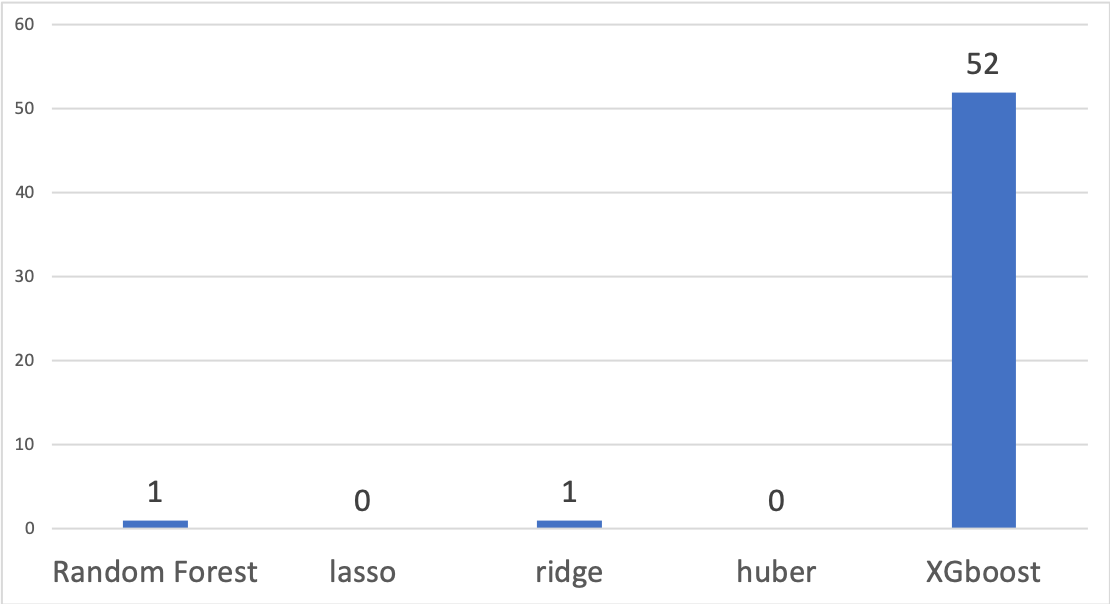
\includegraphics[width=\linewidth]{compare2.png}
\caption{Model provide least MSE}
\label{fig:results}
\end{figure}

\noindent
The distribution of MSE can be seen in Table 3 and Figure 18. The random forest model and linear models have similar MSE distributions while XGBoost has the distribution that concentrated on smaller MSE than the random forest and linear models. In other words, XGBoost can better predict the stock price than other models we selected.

\begin{table}[hbt]
\caption{Table of MSE distribution}
\centering
\begin{tabular}{m{1cm}<{\centering}|m{1.5cm}<{\centering}|c|c|c|c}
MSE range & Random Forest & Lasso & Ridge & Huber& XGBoost \\
\hline
$(0,0.5]$ & 0&0&0&1&0 \\
$(0.5,1]$ & 0&0&0&0&5\\
$(1,1.5]$ & 3&3&2&2&9 \\
$(1.5,2]$ & 7&6&8&7&13 \\
$(2,2.5]$ & 11&10&10&9&16 \\
$(2.5,3]$ & 19&19&18&17&6 \\
$(3,3.5]$ & 4&6&6&6&5 \\
$(3.5,4]$ & 7&5&5&6&0 \\
$(4,4.5]$ & 3&4&4&3&0 \\
$(4.5,5]$ & 0&1&0&1&0
\end{tabular}
\label{tab:label}
\end{table}

\begin{figure}[ht]\centering
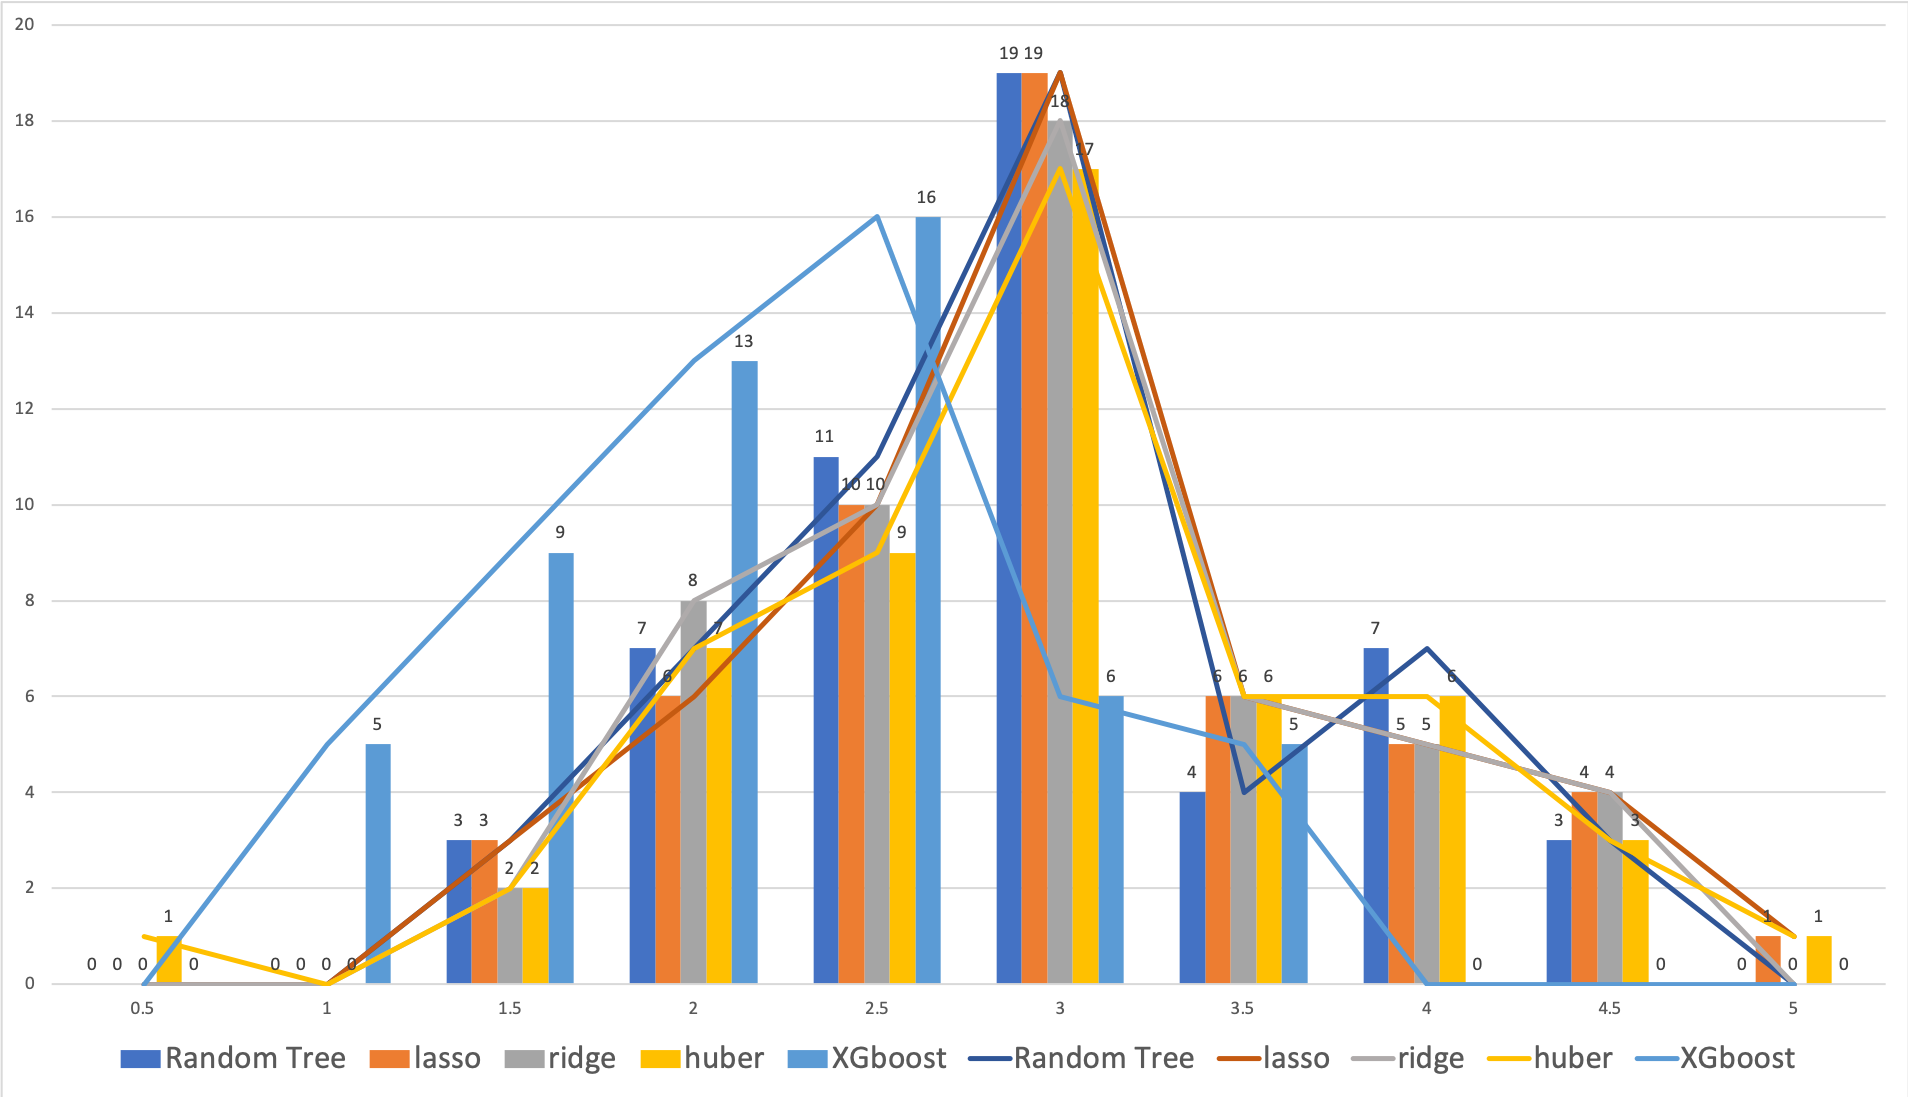
\includegraphics[width=\linewidth]{compare2_2.png}
\caption{MSE distribution}
\label{fig:results}
\end{figure}

\section{Conclusion}
In this project, we utilized various data exploratory method, created 16 features from original dataset, selected features by feature engineering and developed five models, three of which from the class. Then, we compared each model's MSE with testing dataset to understand the characters of each model.\\
\\
\noindent
At first, we used linear models with three different regulator and random forest model to predict stock price. The result turned out that the MSE of these models distributed relatively similar and random forest model performed better than other models. Then, we introduced XGBoost model to improve prediction process. And the result turned out that XGBoost greatly improved the accuracy of stock price. Then, we compared each model and try to explain the reason of the difference among models. \\
\\
Even though XGBoost model has some drawbacks such as less explanatory than linear regression and time-consuming parameter regulation process. XGBoost provides a relatively accurate stock price prediction in our project.\\
\newline
\noindent
However, if our model is widely used in the market, the stocks whose prices we predict to increase is more likely to increase in the future since there would be more people buying it. That is what we called \textbf{Weapon of Math Destruction} problem. The increasing demand will make the stock price grow even more. In that case, the capital will be "locked" in the good stocks in our prediction. That would make the companies with bad performance in the past have less chance to succeed in the future.\\
\newline
\noindent
But that should not be a severe problem. The assumption of the current trading will not affect the price appeared in many economics models and are proved to be effective. Especially for the stock in S\&P 500, whose liquidity is almost the highest ones in the stock market. Also, according to the arbitrage theory, the arbitrage opportunity gradually disappear as more and more participators knowing it. The stock price will be close to its intrinsic value in the long run.\\
\newline
\noindent
In this project, we successfully predict the stock price with several models and find the optimal one. We believe XGBoost could work effectively in real world. And in this project, we only use stock price and trading volumes features. If we add more features such as macro-economy and sentimental factors, we believe our model would perform even better. We believe that financial market practitioners can develop more accurate prediction based on our project. 



%----------------------------------------------------------------------------------------
%	REFERENCE LIST
%----------------------------------------------------------------------------------------
\phantomsection
\bibliographystyle{unsrt}
\bibliography{sample.bib}

%----------------------------------------------------------------------------------------

\end{document}
